\chapter{Introduction}

Insert something about the first responders here, similar to the abstract. Say how the first responders need better tooling for situational awareness, and how the tooling they use currently is inadequate. This can probably be pulled directly from the video here, and cited accordingly, or from some of the other DARPA documentation. Shame the closing ceremony wasn't livestreamed ...

https://www.youtube.com/watch?v=4I4J67jxODE

https://www.darpa.mil/program/darpa-subterranean-challenge

"New York city with the fire department, we have many challenges with the underground subterranean environment, whether it be a train fire, a terrorist incident, or just a derailed train, we don't get that situational awareness of what's going down in the tunnel, what's happening, until we get some firefighters down there"

insert some brilliant transition into talking about how there's an opportunity to address theses challenges, and the rest of the work was done in the context of solving the situational awareness problem for the subt challenge

\section{The DARPA Subterranean (SubT) Challenge}

insert some boilerplate about what the darpa subt challenge is. This is probably a good time to include a few screenshots from their videos which show the various environments. Briefly mention the challenges that need to be addressed. Perception, mobility, communications, autonomy, whatever else.

Also, mention that this is split into a few rounds, and that here we're only focusing on the Tunnel circuit for both development and evaluation, since we don't really know what's coming next. That also lets me be more specific about what artifacts are being used, how much time we have, etc.

Now, talk about the specifics of the perception challenge. Here's some text from the competition rules document:

https://subtchallenge.com/resources/SubT\_Challenge\_Tunnel\_Rules.pdf

Also here's the artifacts specification which we should probably mention here:

https://subtchallenge.com/resources/SubT\_Tunnel\_Artifacts\_Specification.pdf

The main scoring objective is the need to search for, detect, and provide spatially referenced
locations of artifacts relevant to each of the three subdomains. These artifacts could vary in their
size, quantity, and detection signatures (e.g., visual, thermal, chemical). DARPA will announce
the final artifacts in advance of each Circuit Event as part of the finalized event rules
(approximately 90 days before each event) so teams will know what to look for, but the locations
and distribution of the artifacts within the course will not be known. It is expected that the number
of artifacts will be in the range of 10-30 and multiple copies of each artifact type are possible. The
total number of artifacts, but not the number of each type, will be disclosed to the competitors.
The perception problems of interest in the SubT Challenge are focused on the difficulties of
sensing in low-/no-light, obscured, and/or scattering environments. The detection and/or
recognition tasks may benefit from multimodal sensing approaches. Various sensor modalities
and combinations are allowed, including but not limited to: visual, light detection and ranging
(LIDAR), thermal, acoustic, radio frequency (RF), and multi-gas sensors. For example, the
detection of a survivor could potentially be made using a combination of visual, thermal, and/or
auditory cues.

Specifically:

\textbf{Goal:} Report the locations and classes of 20 unique artifacts to DARPA within the competition period (1 hour) within an absolute Euclidean error of 5m.

\textbf{Scoring:} The score is the number of artifacts correctly classified and localized to within 5m of the actual surveyed location by DARPA.

\textbf{Interesting subt specifics (which make it a somewhat different CV problem):}
\begin{itemize}
	\item There are a fixed number of object categories, but the objects within each category are also fixed. That is, there's only 1 survivor, 1 fire extinguisher, etc. List each of the 5 artifacts here.
	\item You're allowed to have a human operator interface with the system. This gives the possibility of using the human in the artifact localization system.
	\item We get (an average of) 2 reports per artifact, so it doesn't have to be correct immediately. Not sure if this is useful here since all the evaluation is performed as if there's only 1 guess. Maybe this could be treated as "immediate" and "final", which is roughly when the guesses would be anyway. This point should be made such that the reader understands that we can continuously update the position, and it's only the final, submitted position that actually has value.
	\item The environment will be foggy / dusty in some places. Also lighting can vary, but that's true for any CV problem ... this probably isn't special
\end{itemize}

TODO: Maybe talk about what's special about each of the artifacts? Namely, Randy has thermal (and is wearing the clothing shown), and the cell phone will have all of its radios on (with specific name for the wifi network being broadcast).

Also, talk about what the localization point means in each of these images. See Figure \ref{randy} for more information.

\begin{figure}
	\centering
	\begin{subfigure}{0.3\textwidth}
		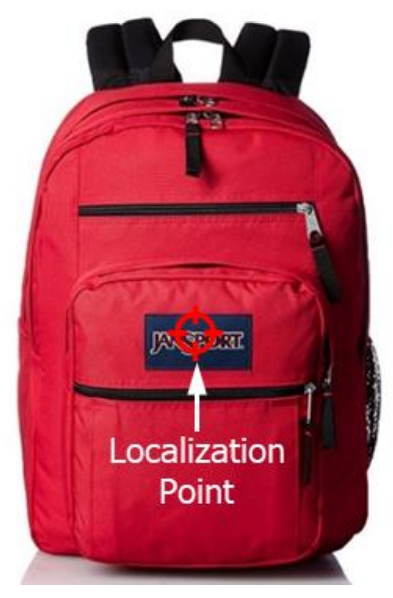
\includegraphics[width=\textwidth]{backpack_artifact.png}
		\caption{Backpack Artifact}
		\label{backpack}		
	\end{subfigure}
	\hfill
	\begin{subfigure}{0.3\textwidth}
		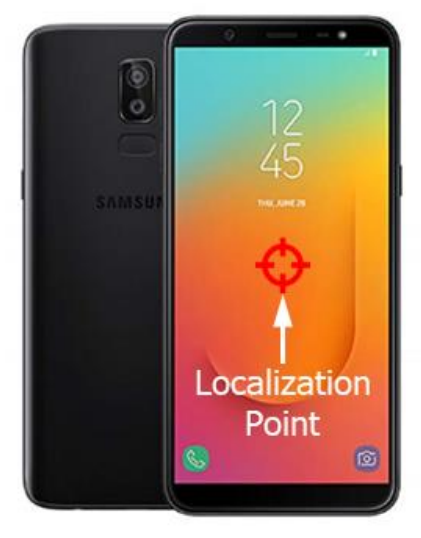
\includegraphics[width=\textwidth]{cell_phone_artifact.png}
		\caption{Cell Phone Artifact}
		\label{cell phone}
	\end{subfigure}	
	\hfill
	\begin{subfigure}{0.3\textwidth}
		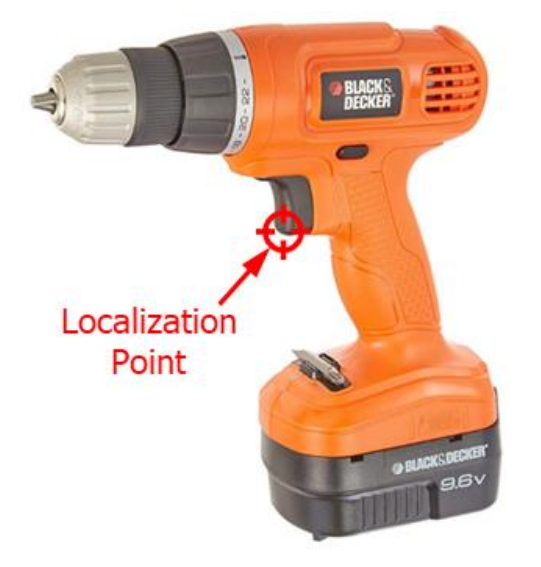
\includegraphics[width=\textwidth]{drill_artifact.png}
		\caption{Drill Artifact}
		\label{drill}
	\end{subfigure}
	\\
	\begin{subfigure}{0.45\textwidth}
		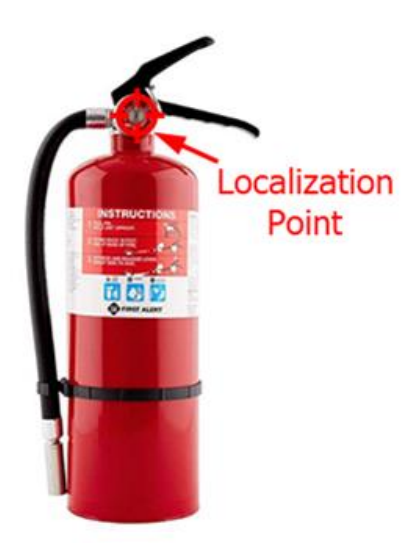
\includegraphics[width=\textwidth]{fire_extinguisher_artifact.png}
		\caption{Fire Extinguisher Artifact}
		\label{fire extinguisher}
	\end{subfigure}	
	\hfill
	\begin{subfigure}{0.45\textwidth}
		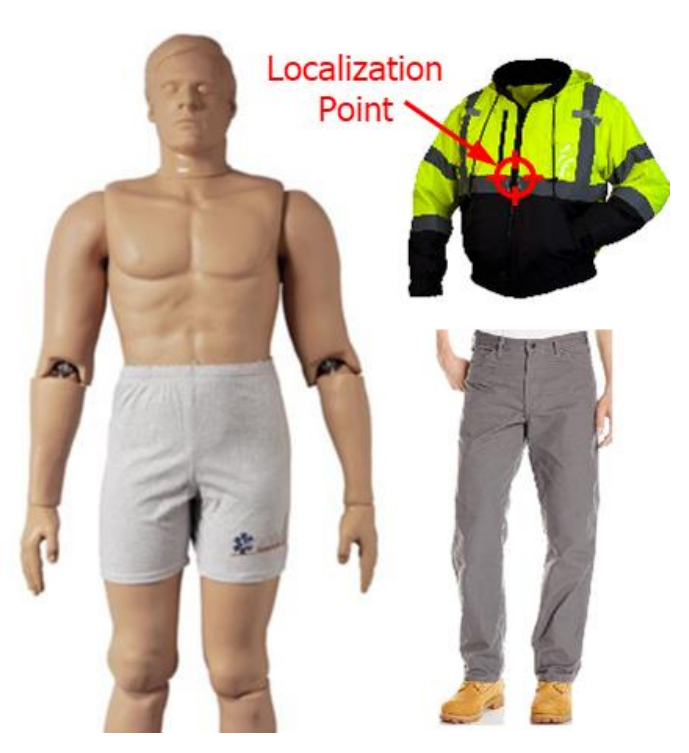
\includegraphics[width=\textwidth]{randy_artifact.png}
		\caption{Survivor Artifact ("Randy")}
		\label{randy}
	\end{subfigure}	
	\caption{Tunnel circuit artifacts}
	\label{tunnel artifacts}
\end{figure}

\section{Related Work}